\documentclass[]{report}
\usepackage{graphicx}
\graphicspath{{images/}}

% Title Page
\title{Conduction, Convection, and Radiation Analysis of an Absorber Plate for a Solar Water Heater}
\author{Caleb J. Groves}


\begin{document}
\maketitle

\begin{abstract}
\end{abstract}

\section{Introduction}

There is a strong push today to develop more environmentally-friendly ways of generating and using energy. One of the most available and interesting sources of alternative energy is solar energy. While solar energy is abundant, it tends to be of a lower grade than other forms. As such, the harvesting of this energy should be done as efficiently as possible in order to maximize the output which is needed for various applications.

This analysis compares the efficiencies of two designs for a solar water heater: one with a convection shield, and one without. The objective is to determine whether one design has a significant advantage over the other in terms of energy efficiency. The analysis is carried out using fundamental laws and principles of thermodynamics and heat transfer in order to develop a model of the solar water heater under both shielded and unshielded conditions. This model is then used to predict values for the efficiencies of the designs and give recommendations based on the results.

\section{Methods}

% General approach: identify the system, develop differential equation to model system, solve equation, solve specifically for convection and radiation terms, use given values to analyze numerically and derive results.
We define the efficiency of the solar water heater as the ratio of the rate energy is transferred to the water to the rate solar energy is incident on the absorbing surface. The general approach to analyzing the efficiencies of the two designs is as follows: the system is identified and used to develop differential equations in order to model it. This equation is then solved to obtain a the temperature profile along the absorber plate, and this temperature distribution is then used to obtain expressions for the rate energy is transferred to the water. Specific terms in these equations are solved for on a more detailed level, and then these expressions are evaluated numerically to obtain results.

\subsection{Schematic}

A general schematic for the problem is shown below in Fig. \ref{fig:base_schematic}, including values which we will assume are accurate. The solar water heater is exposed to a uniform solar flux $q''_{solar}$ at an angle $\theta$ relative to the surface normal, and quiescent air at temperature $T_{\infty}$. The bottom of the absorber plate is insulated, and the plate itself has a diffuse, spectrally selective coating with the spectral reflectivity shown in Fig. \ref{fig:base_schematic}. The water circulating through the tubes is assumed to keep the absorber plate directly above each pipe at $T_0$. We will model the surroundings as large and isothermal, also at $T_{\infty}$.

\begin{figure}[h]
	\centering
	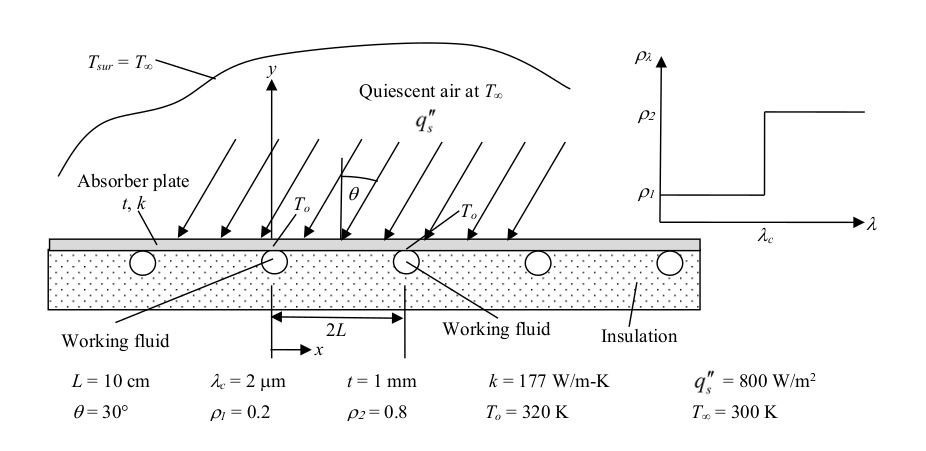
\includegraphics[width=8cm]{schematic1.png}
	\caption{Schematic of the solar water heater and its interactions with the environment.}
	\label{fig:base_schematic}
\end{figure}

\subsection{Assumptions}

\subsection{Analysis}

\subsubsection{System Modeling}

Since we will need to know the temperature distribution in the absorber plate in order to determine the efficiency of the heat transfer to the water, we will choose our system to be a differential control volume in the absorber plate and model the energy interactions of this control volume with the surroundings, as shown in Fig. \ref{fig:model_schematic}.

\begin{figure}[h]
	\centering
	%\includegraphics[width=8cm]{modeling_schematic.png}
	\caption{Schematic of a differential control volume of the system of interest (the absorber plate), and the energy interactions of that system with its surroundings.}
	\label{fig:model_schematic}
\end{figure}

\section{Results}

\section{Discussion}

\end{document}          
